\section{Introducción.}
Recordando, un servidor DHCP es un servidor que recibe peticiones de clientes solicitando una configuración de red IP. El servidor responderá a dichas peticiones proporcionando los parámetros que permitan a los clientes autoconfigurarse. Para que un PC solicite la configuración a un servidor, en la configuración de red de los PCs hay que seleccionar la opción 'Obtener dirección IP automáticamente'.\\

El servidor proporcionará al cliente al menos los siguientes parámetros: 
	
	\begin{itemize}
		\item Dirección IP.
		\item Máscara de Subred.
	\end{itemize}
	
Opcionalmente, el servidor DHCP podrá proporcionar otros parámetros de configuración tales como:


	\begin{itemize}
		\item Puerta de enlace 
		\item Servidores DNS
		\item Muchos otros párametros más
	\end{itemize}
	
\section{Definiciones.}	

Antes de comenzar con los procesos de instalación y configuración de nuestro servidor DHCP, vamos a definir algunos términos que utilizaremos a lo largo de dicho proceso. \\
\\

\textbf{Ámbito servidor DHCP: } Un ámbito es un agrupamiento administrativo de equipos o clientes de una subred que utilizan el servicio DHCP.\\
\\
\textbf{Rango servidor DHCP: } Un rango de DHCP está definido por un grupo de direcciones IP en una subred determinada, como por ejemplo de 192.168.0.1 a 192.168.0.254, que el servidor DHCP puede conceder a los clientes.\\
\\
\textbf{Concesión o alquiler de direcciones: } es un período de tiempo que los servidores DHCP especifican, durante el cual un equipo cliente puede utilizar una dirección IP asignada.\\
\\
\textbf{Reserva de direcciones IP: } Consiste en reservar algunas direcciones IP para asignárselas siempre a los mismos PCs clientes de forma que cada uno siempre reciba la misma dirección IP. Se suele utilizar para asignar a servidores o PCs concretos la misma dirección siempre. Es similar a configurar una dirección IP estática pero de forma automática desde el servidor DHCP. En el servidor se asocian direcciones MAC a direcciones IP. Es una opción muy interesante para asignar a ciertos PCs (servidores, impresoras de red, PCs especiales...) siempre la misma IP.\\
\\


\section{Requerimientos.}
	A continuación se hace mención de los requerimientos necesarios para iniciar la instalación.
	\begin{itemize}
		\item Sistema operativo Debian GNU/Linux 7 whezzy.
		\item Tener actualizado los repositorios.
		\item Deshabilitar el DHCP del router a utilizar (módem en su defecto).
		\item Habilitar la IP estática tanto en el servidor como en el módem.
	\end{itemize}		
	
	
\section{Instalación del ISC DHCP.}
En Debian GNU/Linux, el paquete de software que contiene el servidor DHCP de ISC (Internet System Consortium) se denomina isc-dhcp-server y para su instalación procedemos de la siguiente manera (considere antes de ingresar el comando, tener permisos de super usuario)  :
	
	\begin{listing}[style=consola, numbers=none]
	    $apt-get install isc-dhcp-server
 	\end{listing}

	Una vez instalado, como podemos ver a continuación, se intenta automáticamente lanzar el servidor pero da un fallo debido a que aún no hay ninguna configuración establecida.
	
	\begin{listing}[style=consola, numbers=none]
	    $isc-dhcp-server, action "start" failed.
 	\end{listing}

El programa que implementa el servidor DHCP es /usr/sbin/dhcpd y éste, como todos los servicios, lo podremos manejar a través de un script del directorio /etc/init.d/ o bien con el comando service:

	\begin{listing}[style=consola, numbers=none]
# /etc/init.d/isc-dhcp-server
Usage: /etc/init.d/isc-dhcp-server {start|stop|restart|force-reload|status}
# /etc/init.d/isc-dhcp-server start
[ ok ] Starting ISC DHCP server: dhcpd.
 	\end{listing}

La instalación anterior del servidor debe haber configurado el sistema operativo para que se active automáticamente cuando se encienda el ordenador. Esto lo podemos comprobar mirando que exista el fichero que lanzará el arranque (Start) del servidor DHCP, el cual debe encontrarse al menos en el directorio init del nivel de arranque actual de nuestro sistema operativo. Para saber cuál es el nivel de arranque actual usaremos la instrucción who:

	\begin{listing}[style=consola, numbers=none]
	$who -r
	$ls /etc/rc2.d
 	\end{listing}
	
	Como resultado se debe encontrar el archivo S17isc-dhcp-server, con ello aseguramos que se inicie al reiniciar el servidor.\\

Ficheros del servidor DHCP a tener en cuenta son los siguientes:
	\begin{itemize}
		\item /etc/dhcp/dhcpd.conf: es el fichero de configuración del servidor. Se puede modificar con el servidor ejecutándose, y una vez modificado reiniciaremos el servicio.
		\item /var/lib/dhcp/dhcpd.leases: es el fichero base de datos donde se registran todas las concesiones de IP que se van dando a los clientes.
		\item /etc/default/isc-dhcp-server: desde aquí se puede especificar qué ficheros sustituirán a los dos anteriores; también, cuáles serán las interfaces por las que el servidor DHCP escuchará peticiones de IP.
		\item /var/log/syslog: en este fichero se irán escribiendo los mensajes log del servidor DHCP, a menos que lo cambiemos a otro fichero.
		\item /var/run/dhcpd.pid: contiene el PID de servidor DHCP (dhcpd).
		\item /usr/share/doc/isc-dhcp-*: varios directorios donde hay diversa documentación sobre el servicio DHCP junto con ejemplos.
	\end{itemize}		

Podemos usar la orden man para obtener diversa documentación:

	\begin{itemize}
		\item man dhcpd
		\item man dhcpd.conf
		\item man dhcp-options
		\item man dhcp-eval
	\end{itemize}		

\subsection{/etc/default/isc-dhcp-server}
El fichero /etc/default/isc-dhcp-server es el primer fichero de configuración que lee el servidor DHCP (/usr/sbin/dhcpd), y con él podemos cambiar varias cosas que veremos a continuación.

A veces el ordenador donde se encuentra el servidor DHCP tiene más de una interfaz de red, y puede que necesitemos que éste no trabaje por todas las interfaces, es decir, que sólo atienda peticiones por unas cuantas. Para hacer esto debemos modificar la variable INTERFACES. El valor por defecto es el siguiente:

	\begin{listing}[style=texto, numbers=none]
	INTERFACES=""
 	\end{listing}

lo cual indica que el servidor escucha peticiones por todas sus interfaces. Si sólo debe escuchar por las interfaz eth0, pondríamos el siguiente valor:
	\begin{listing}[style=texto, numbers=none]
	INTERFACES="eth0"
 	\end{listing}
 	
La variable DHCPD\_CONF se utiliza para especificar cuál será el fichero de configuración principal (dhcpd.conf) del servidor DHCP. Por defecto se asume:
 	\begin{listing}[style=texto, numbers=none]
	DHCPD_CONF=/etc/dhcp/dhcpd.conf
 	\end{listing}
 	
 	También puede cambiarse el fichero que guarda el PID asignado al proceso del servidor DHCP, esto es a través de la variable DHCPD\_PID, cuyo valor por defecto es:
 	
  \begin{listing}[style=texto, numbers=none]
   DHCPD_PID=/var/run/dhpcd.pid
  \end{listing}
 	
 	El servidor DHCP (/usr/sbin/dhcpd) puede ejecutarse pasándole algunas opciones (-f, -d, -q, -t, etc.), las cuales pueden consultarse ejecutando la orden "man dhcpd". Esta opciones pueden especificarse a través de la variable OPTIONS, que por defecto no lleva ninguna:
  
  \begin{listing}[style=texto, numbers=none]
	OPTIONS="-f -d"
 	\end{listing}

Otra forma sería mediante la ejecución directa del demonio DHCP:
 	
 	\begin{listing}[style=consola, numbers=none]
	$/usr/sbin/dhcpd -f -d
 	\end{listing}
 	%$
 	\subsubsection{Ejemplo del archivo isc-dhcp-server}
 	El ejemplo se muestra en la figura \ref{fig:1}
 	\begin{figure}
  \centering
    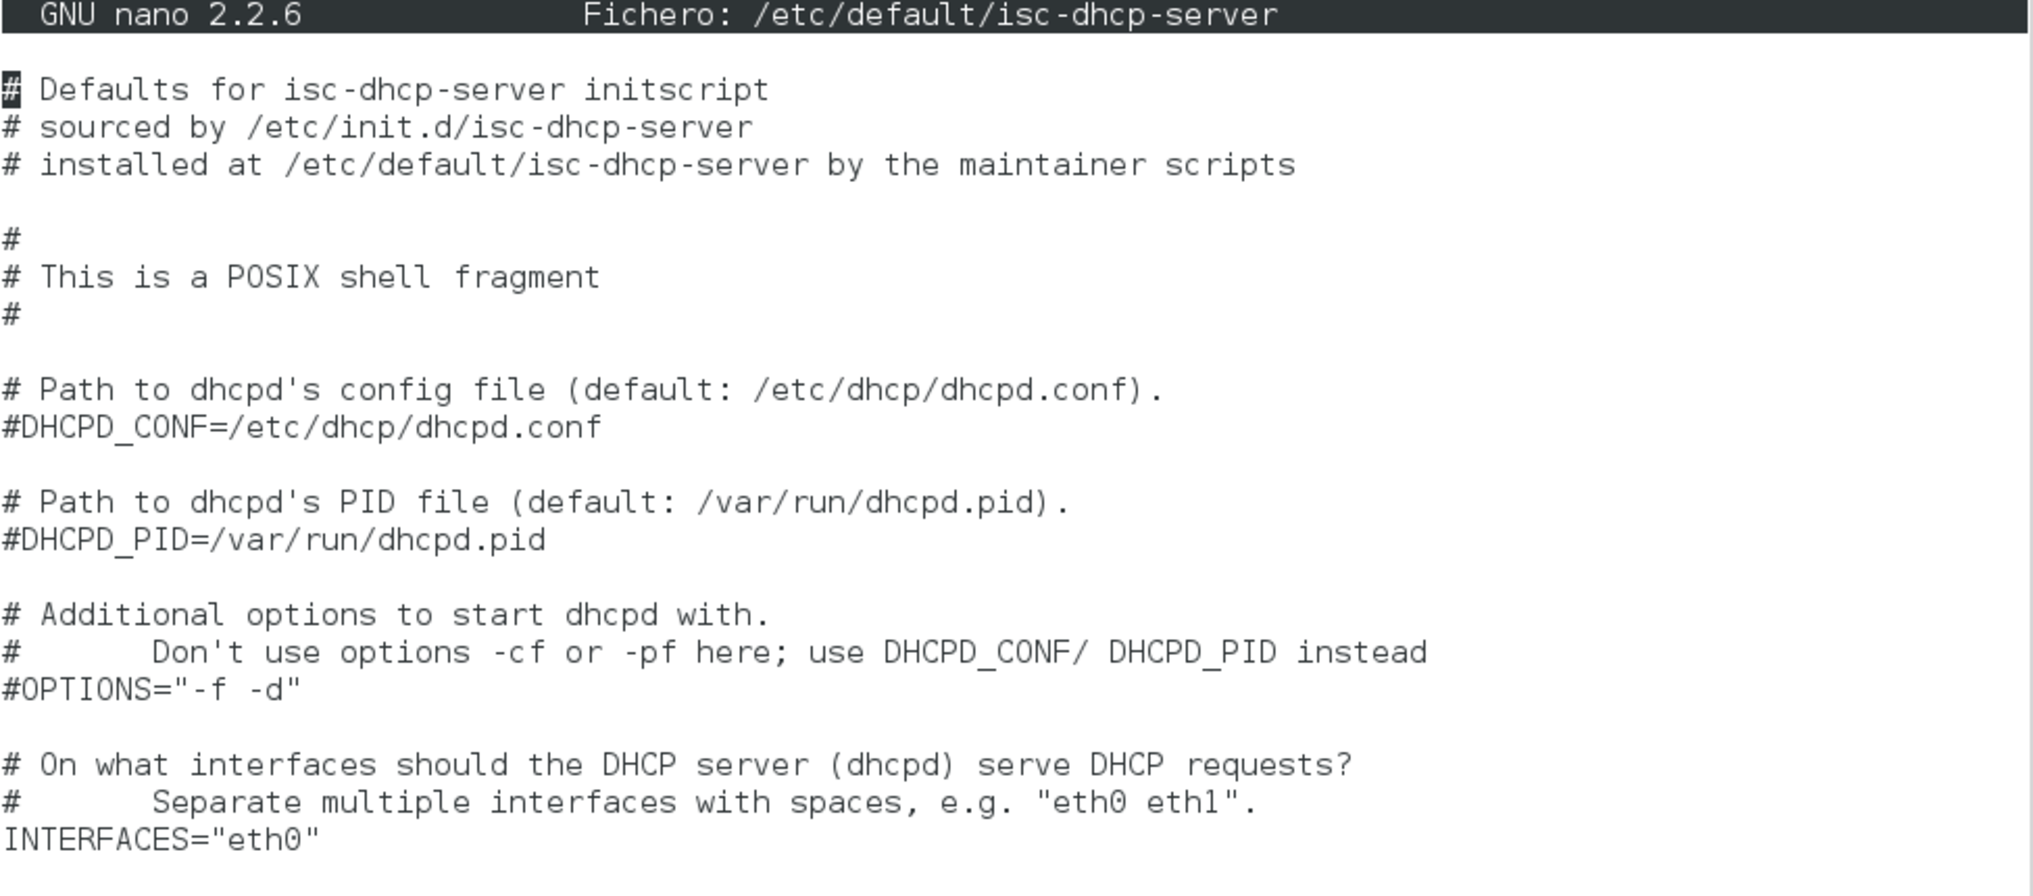
\includegraphics[width=0.7\textwidth]{img/isc-dhcp}
  \caption{isc-dhcp-server}
  \label{fig:1}
\end{figure}
 	
 	\subsection{/var/log/syslog}
 	
 	El servidor ISC DHCP envía mensajes log para indicar múltiples situaciones por las que pasa, que van desde simples informaciones hasta notificaciones de errores. Estos mensajes log, tanto del servidor DHCP como de otros servicios, los maneja el demonio rsyslogd (/usr/sbin/rsyslogd) a través del protocolo SYSLOG, y por defecto acaban en el fichero /var/log/syslog, mezclado con todos los demás mensajes log. Esto último se puede cambiar si estamos interesados en separar los log del servidor DHCP de los demás.
 	
 	Los mensaje log pertenecen a una categoría y poseen una prioridad. Las categorías pueden ser: auth, authpriv, cron, daemon, kern, lpr, mail, mark, news, syslog, user, uucp y local0 hasta local7. Si no se especifica otra cosa, los log del servidor ISC DHCP son de la categoría daemon. Por otro lado, a cada log se le asigna una prioridad, que puede ser una de las siguientes ordenadas de menor a mayor prioridad: debug, info, notice, warning, err, crit, alert y emerg.
 	
 	En el fichero /etc/rsyslog.conf se configura el comportamiento de rsyslogd, indicando entre otras cosas, en qué ficheros se guardan los mensajes log según su categoría y prioridad. Si queremos que los mensajes log del servidor DHCP se guarden en un fichero aparte, seguimos los siguientes pasos:
 	\begin{enumerate}
 		\item En /etc/dhcp/dhcpd.conf añadimos la línea "log-facility local1;", con lo que conseguimos cambiar la categoría de los log del DHCP.
 		\item En el fichero /etc/rsyslog.conf añadimos la línea "local1.info /var/log/dhcp.log" para que todos los log de la categoría local1 y prioridad info o superior se escriban en el fichero /var/log/dhcp.log.
 		\item Creamos el fichero vacío /var/log/dhcp.log, pues rsyslogd no lo crea.
 		\item Reiniciamos los servicios con /etc/init.d/rsyslog y /etc/init.d/isc-dhcp-server.
 	\end{enumerate}
 	Si no hacemos lo anterior, siempre podremos filtrar los mensaje log del DHCP pues estos llevan siempre el texto "debian dhcpd" y por lo tanto ejecutaríamos:
 	
 	 \begin{listing}[style=consola, numbers=none]
	$fgrep "debian dhcpd" /var/log/syslog
 	\end{listing}
 	%$
 	El servicio rsyslogd es muy potente y una de sus mejores cualidades es la de centralizar todos los log de diversas máquinas de una red en una serie de ficheros situados en un único ordenador, el protocolo SYSLOG no se tratará en este documento. 
 	 
 	 \subsubsection{Ejemplo del archivo syslog}
 	 El ejemplo se muestra en la figura \ref{fig:2}
 	\begin{figure}
  \centering
    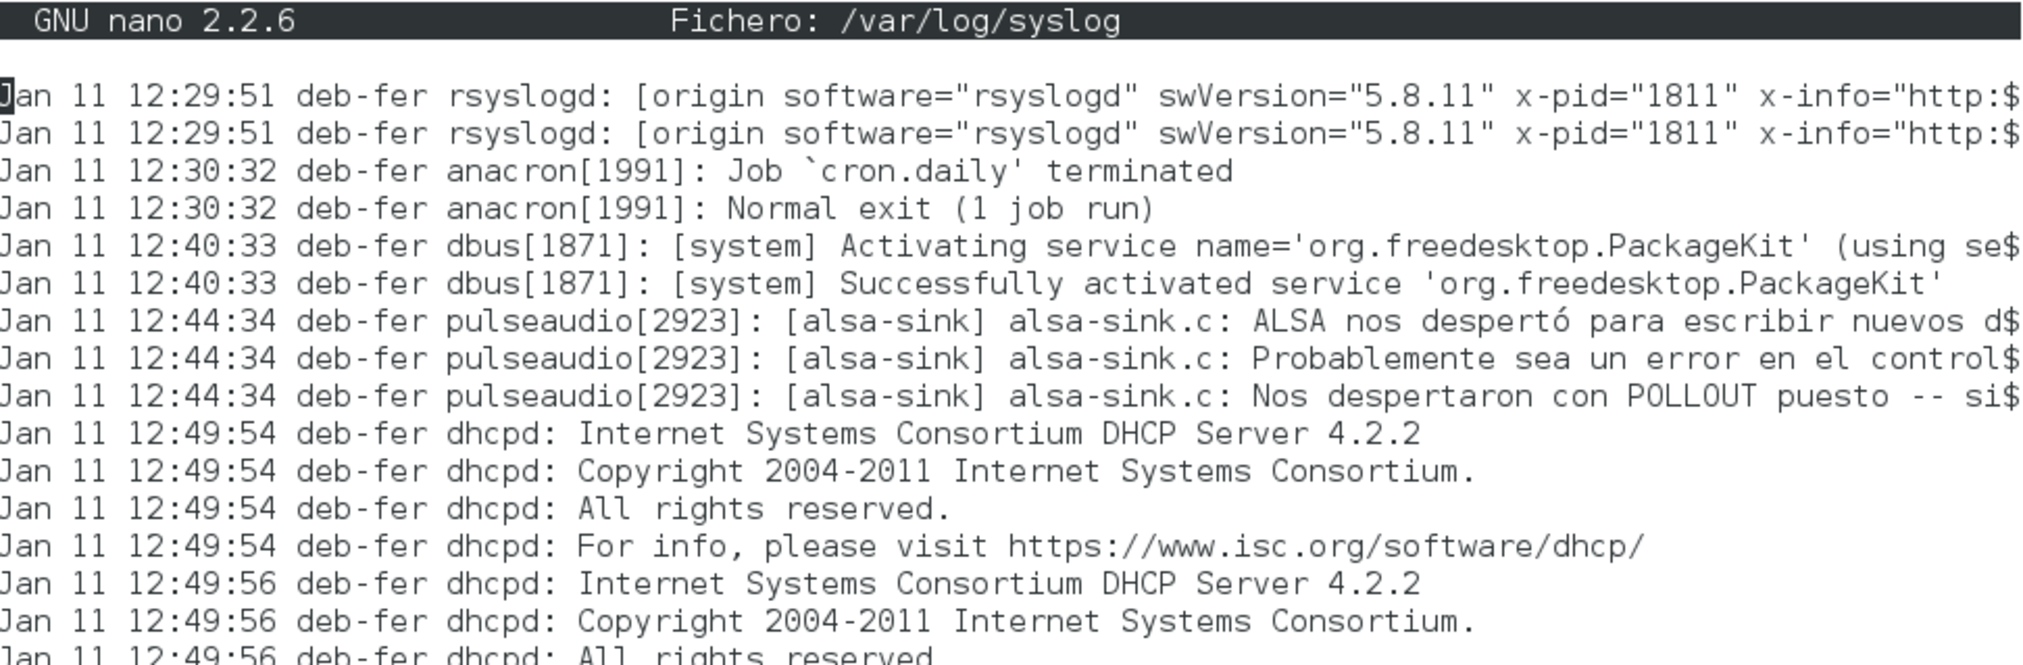
\includegraphics[width=0.7\textwidth]{img/syslog}
  \caption{syslog}
  \label{fig:2}
\end{figure}
 
 \section{/etc/dhcp/dhcpd.conf}
 Como ya se ha dicho, en el fichero /etc/dhcp/dhcpd.conf es donde se especifica cómo va a funcionar el servidor ISC DHCP. En este punto se va a explicar el papel que cumplen muchas de las distintas declaraciones y estamentos que podemos escribir en él.

Algunos convenios de este fichero son los siguientes:	

\begin{itemize}
	\item[\#] comienza un comentario hasta el final de la línea y puede ponerse en cualquier lugar.
	\item No se distingue entre mayúsculas y minúscula.
	\item Todos los estamentos deben acabar con el signo de punto y coma (;). Las declaraciones que definen un ámbito mediante los signos { y } no finalizan en punto y coma.
\end{itemize}
 	
 	\subsection{Ejemplo de configuración del archivo dhcpd.conf}	
 	El ejemplo se muestra en la figura \ref{fig:3}
\begin{figure}
  \centering
    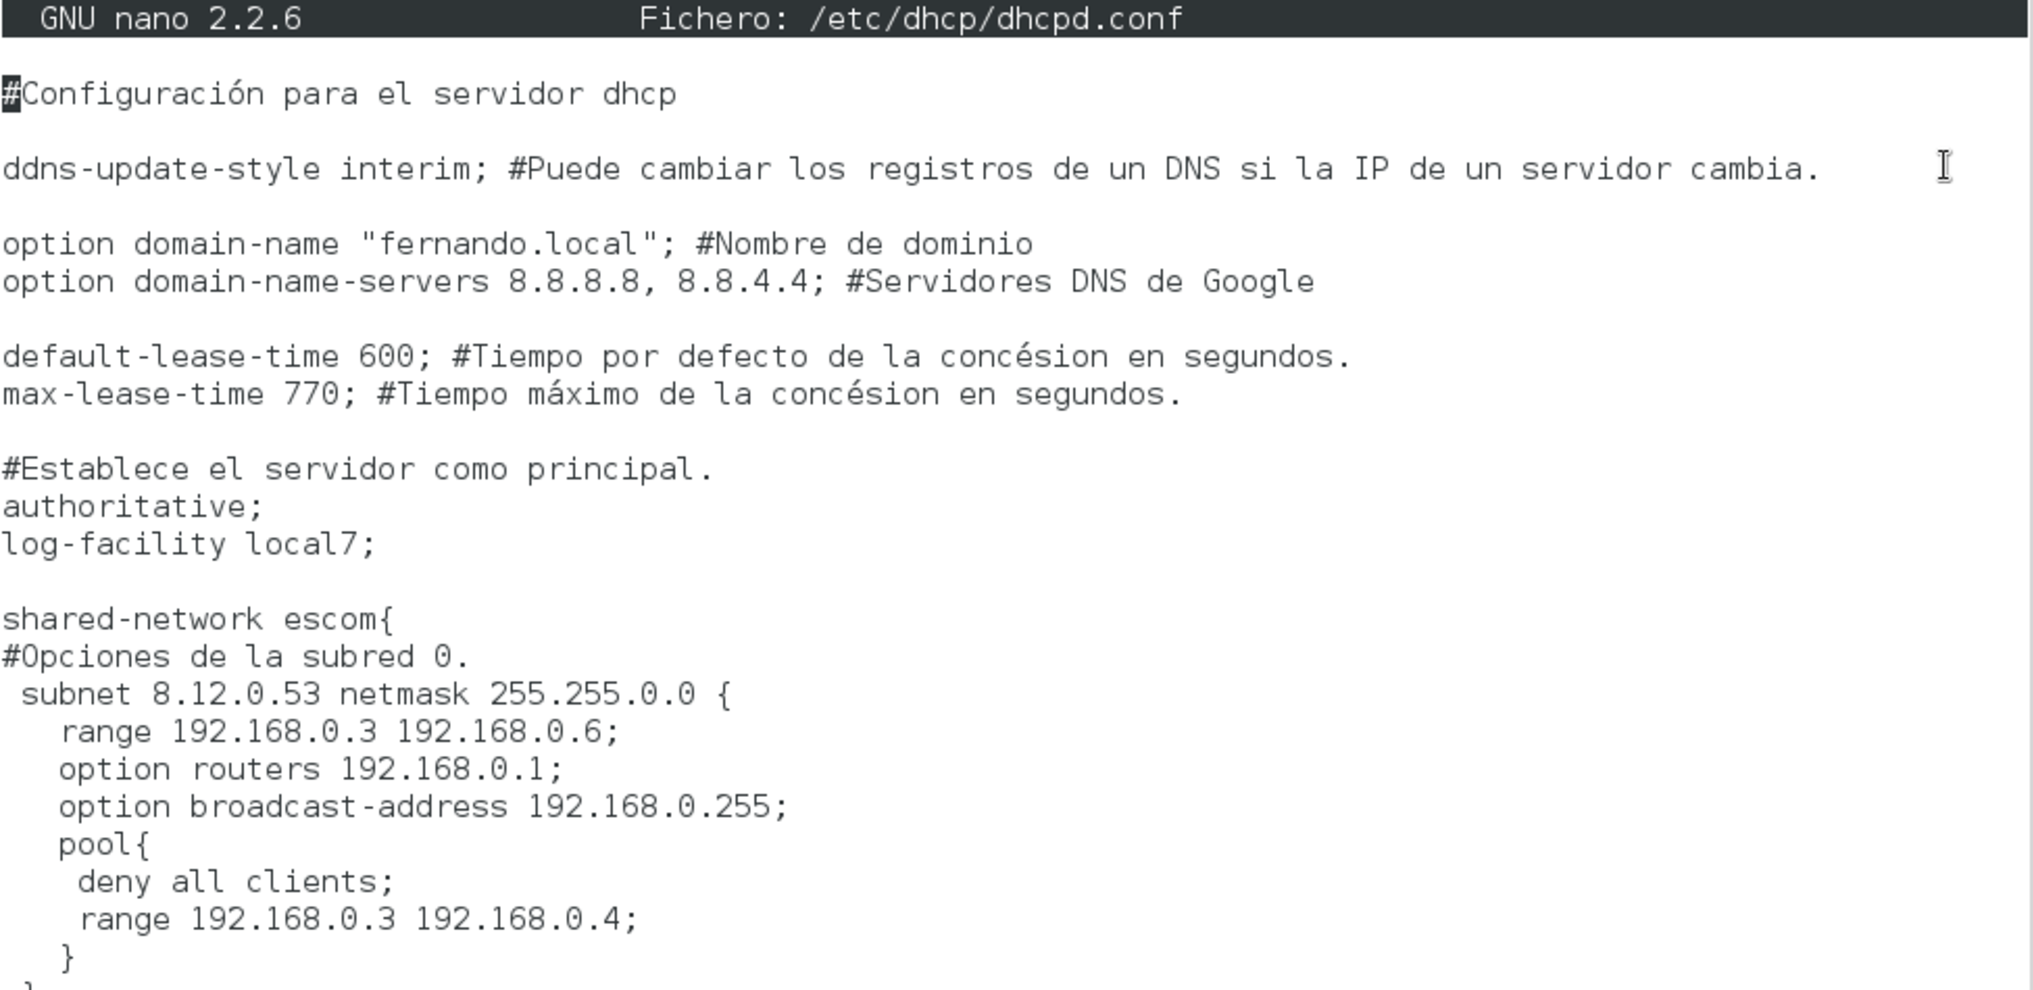
\includegraphics[width=0.8\textwidth]{img/dhcp1}
    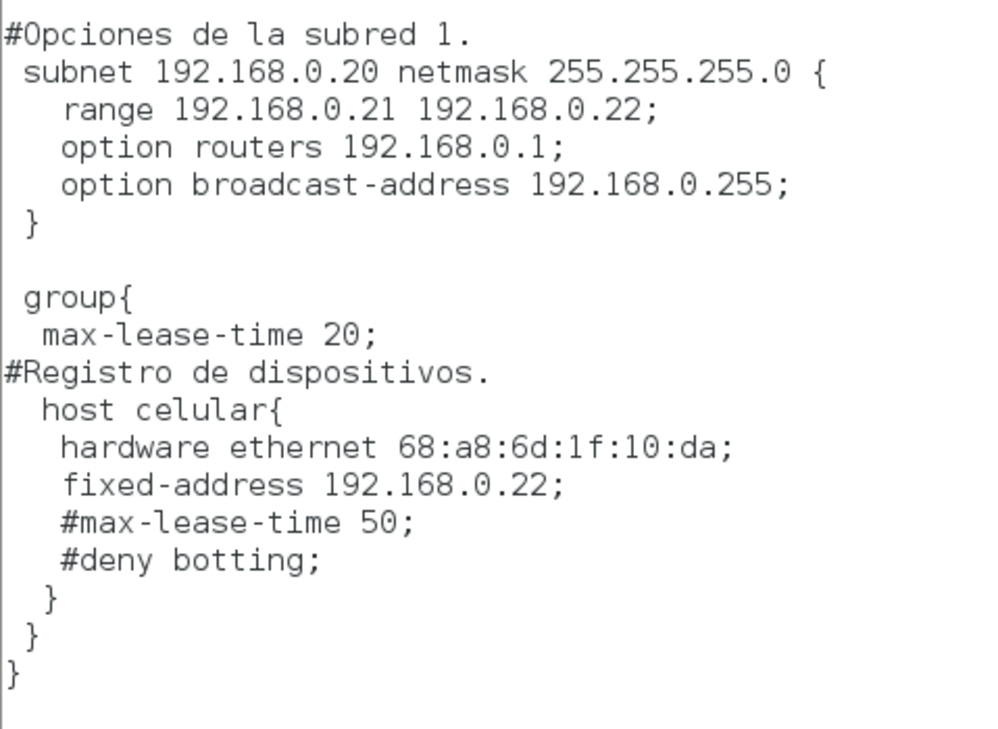
\includegraphics[width=0.5\textwidth]{img/dhcp2}
  \caption{dhcp}
  \label{fig:3}
\end{figure}
En el documento se muestran algunos de los elementos tales como:
\subsubsection{authoritative}
Definir el estado del parámetro authoritative es lo primero que deberíamos hacer en una configuración de un servidor DHCP. Si un servidor es autoritario entonces podrá enviar mensajes DHCPNACK a aquellos clientes que envían un DHCPREQUEST con una propuesta de IP no válida, debido a que al cliente se le ha cambiado de segmento de red. En estos casos, si el servidor no es autoritario, lo que hace es no contestar.

\subsubsection{ddns-update-style}
El parámetro ddns-update-style se utiliza para especificar si el servidor DHCP hará actualizaciones DNS del nombre del cliente junto con la asignación de la IP. Su sintaxis es la siguiente: \textbf{ddns-update-style estilo;}\\

El valor de estilo será uno de los siguientes:
\begin{itemize}
	\item none: para indicar que no hará actualizaciones DNS.
	\item ad-hoc: es un estilo de sincronización entre los servidores DHCP y DNS. No es recomendado este estilo.
	\item interim: es el estilo de sincronización recomendado.
\end{itemize}

\subsubsection{shared-network}
Como ya se ha mencionado, en ocasiones a un segmento de red se le asignan más de una subred, y para que el servidor DHCP sea consciente de esto, lo que hay que hacer es agrupar en el ámbito de una declaración shared-network las distintas declaraciones subnet que definen las subredes.

\subsubsection{range}
La declaración range se utiliza para especificar el rango de IP que una subred tiene disponible para servir a sus clientes. En una declaración subnet pueden ponerse una o más declaraciones range y todas las direcciones IP especificadas deben pertenecer a la red de subnet.

\subsubsection{option domain-name-servers}
La opción domain-name-servers se emplea para enviar al cliente los servidores DNS que utilizará. Su sintaxis es la siguiente: option domain-name-servers ip-address [, ip-address...  ];\\
Los servidores se deben especificar por orden de preferencia, siendo el primero de la lista el que se utilizará como servidor DNS primario.

\subsubsection{host}
La declaración host se utiliza para especificar la información a asignar a un cliente DHCP concreto.

\subsubsection{group}
La declaración group se utiliza para crear ámbitos, por ejemplo, podría utilizarse para agrupar un conjunto de declaraciones host y definir sólo una vez los parámetros comunes.

\section{Configuración de red}

	Una vez que se ha creado el esquema necesario para proporcionar las ip a nuestras redes se debe proceder a configurar las ip estáticas dentro del archivo de interfaces ubicado en /etc/network/interfaces, lo configuramos de tal forma que le asigne una ip puesto que al módem se le ha des-habilitado la funcionalidad de dhcp, de igual forma en la configuración del punto de acceso se debe configurar esta ip.
	El ejemplo para la configuración se muestra en la figura \ref{fig:4}
	\begin{figure}
  \centering
    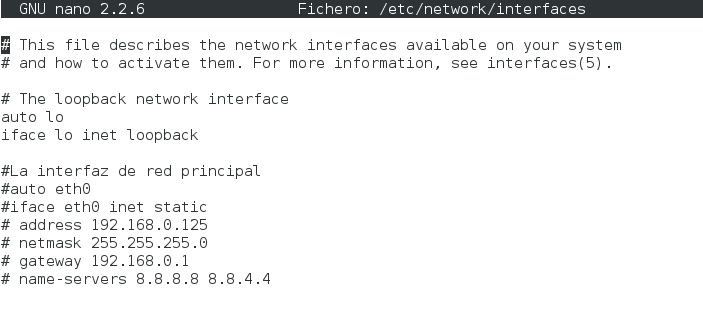
\includegraphics[width=0.8\textwidth]{img/interfaces}
  \caption{interfaces}
  \label{fig:4}
\end{figure}

\section{Activación del servicio}

Al momento de tener configurado y actualizado todos los ficheros antes mencionados se procede a levantar los servicios de la siguiente manera:
\begin{enumerate}
	\item Levantar la interfaz de red
	 	\begin{listing}[style=consola, numbers=none]
	$/etc/init.d/networking restart
 	\end{listing}
 	%$
 	\item Levantar el servidor dhcp
 	\begin{listing}[style=consola, numbers=none]
	$/etc/init.d/isc-dhcp-server restart
 	\end{listing}
 	%$
\end{enumerate}

Con los pasos anteriores tenemos nuestro servidor dhcp en funcionamiento.

\section{Monitoreo}
Para poder administrar el servidor contamos con ciertas herramientas para cumplir la tarea:

\begin{itemize}
	\item Verificar que la interfaz seleccionada tenga la ip asignada
	\begin{listing}[style=consola, numbers=none]
	$ifconfig
 	\end{listing}
 	%$
 	\item Verificar el registro de los clientes al servidor en el archivo /var/lib/dhcp/dhcp.leases.
 	\item Verificar las peticiones en el log, expuesto en las primeras secciones.
 	\item Hacer uso de herramientas para una mejor administración de los log del servidos.
\end{itemize}

